\documentclass[12pt,a4paper]{article}

\usepackage[fleqn]{amsmath} % This package with the fleqn option aligns equations to the left
\setlength{\mathindent}{0pt} % Set indentation from the left margin

\usepackage{amssymb} % Required for math symbols
\usepackage{graphicx} % Required for inserting images
\usepackage{geometry}

\usepackage{booktabs}  % For professional looking tables
\usepackage{longtable} % For tables that might span multiple pages

\usepackage{multirow}

\usepackage[backend=biber, style=authoryear, citestyle=authoryear]{biblatex}
\addbibresource{references.bib}

\geometry{a4paper, margin=1in}

{
\title{
    
\includegraphics[width=0.34\textwidth]{/Users/mlnick/documents/images/tsukuba-logo.png} \\
    \vspace{2mm}
    \textbf{Experiment Design in Computer Science} \\
    \vspace{3mm}    
    Report 2: Comparative Analysis of   \\
    Differential Evolution Algorithms   \\
    Under Varied Configuration Settings
}

\author{Mamanchuk Mykola, SID.202420671}
\date{\today}
}

\usepackage{listings}
\usepackage{color}

\definecolor{codegreen}{rgb}{0,0.6,0}
\definecolor{codegray}{rgb}{0.5,0.5,0.5}
\definecolor{codepurple}{rgb}{0.58,0,0.82}
\definecolor{backcolour}{rgb}{0.99,0.99,0.99}

\lstdefinestyle{mystyle}{
    backgroundcolor=\color{backcolour},   
    commentstyle=\color{codegreen},
    keywordstyle=\color{magenta},
    numberstyle=\tiny\color{codegray},
    stringstyle=\color{codepurple},
    basicstyle=\ttfamily\footnotesize,
    breakatwhitespace=false,         
    breaklines=true,                 
    captionpos=b,                    
    keepspaces=true,                 
    numbers=left,                    
    numbersep=5pt,                  
    showspaces=false,                
    showstringspaces=false,
    showtabs=false,                  
    tabsize=2
}
\lstset{style=mystyle}

\setlength{\fboxsep}{0pt} % Removes padding around the image
\setlength{\fboxrule}{0.5pt} % Sets the thickness of the border

\begin{document}

\maketitle

% #################### STARTING HERE ####################

\section{Abstract}
Upon studying the differential evolution (DE) algorithms using statistical techniques, this report evaluates the influence of parameter tuning on algorithm performance. The primary objective was to assess different DE configurations by manipulating parameters such as the number of benchmarks, repetition counts, Differential Weight (F), and Crossover Probability (Cr). It was found that all three selection policies exhibit statistically significant differences when specific parameter sets are applied and a substantial data volume is collected, enabling precise analysis. The findings suggest that parameter tuning plays a crucial role in the performance of DE algorithms, with some observations raising questions for further analysis. This report aims to present these findings systematically, providing a basis for more detailed investigations into DE algorithm optimization.

\section{Introduction}
\subsection{Background}
DE is a robust, population-based optimization algorithm commonly used to solve complex multi-dimensional functions that are otherwise challenging for traditional optimization methods. It relies on mechanisms of mutation, crossover, and selection to evolve solutions toward an optimum. The effectiveness and efficiency of DE can significantly vary based on its parameter settings: these parameters control the perturbation of vectors and the recombination process, respectively, playing crucial roles in the convergence behavior of the algorithm.

This report explores DE within the framework of the CEC 2014 optimization benchmark set, which provides a diverse set of problems to test the adaptability and efficiency of evolutionary algorithms.

\subsection{Objectives}
The primary objective is to systematically analyze how different configurations of the DE algorithm influence its performance. This involves a comparative analysis of three distinct selection policies:
\begin{itemize}
    \item \textbf{Select Best:} Focuses on selecting the best solution vectors for mutation and crossover, promoting rapid convergence.
    \item \textbf{Select Random:} Employs a random selection strategy, enhancing diversity in the population but potentially slowing convergence.
    \item \textbf{Select Random-to-Best:} A hybrid approach that mixes the best vector with random selections to balance exploration and exploitation.
\end{itemize}

Further, the report discuses:
\begin{enumerate}
    \item Evaluate fine-tuning of parameters F and Cr on each selection policy to discern optimal settings for different types of optimization problems.
    \item Determine the statistical significance of observed differences in performance by employing robust statistical techniques.
    \item Estimate the required sample size and calculate power to ensure that the experimental design can reliably detect a practical difference, if one exists, between the configurations.
\end{enumerate}

\newpage

\section{Methodology}

\subsection{Experimental Setup}
The experimental setup is outlined as follows:

\vspace{3mm}

\textbf{Software:}
\begin{itemize}
    \item Primary platform: Python v3.12.2
    \item Utilized libraries include pygmo, pandas, seaborn, matplotlib, scipy, statsmodels, itertools, numpy, scikit\_posthocs, and other standard packages.
    \item Development environment: Visual Studio Code v1.91.0
    \item Operating System: MacOS 13.6.7 22G720 x86\_64
\end{itemize}

\textbf{Hardware:}
\begin{itemize}
    \item Processor: Intel i7-7920HQ 8 @ 3.10GHz
    \item Memory: DRAM LPDDR3 2133MHz 16GB
\end{itemize}

\textbf{Utilized Scripts:}
\begin{itemize}
    \item \texttt{base\_script.py} [2]: Provided as part of the assignment. Implements essential steps for data collection. This script was modified for semi-automatic output of data in a convenient way to create many distinct collections of individual experiments. It also provides information on individual algorithm's runtime.
    \item \texttt{all\_stats.py} [2]: Main supplement, which implements statistical calculations, testing, validation, plotting, and file management essentials in a convenient way.
    \item \texttt{sample\_size.py} [2]: Supplementary script used to calculate hypothetical sample size based on conditions stated in the task by simulating the Kruskal-Wallis non-parametric method. Also available in Appendix A.
    \item \texttt{record\_performance\_and\_runtime.py} [2]: Supplementary script that takes out best cases for performance for Selection Policies based on F and CR and outputs into a file; outputs runtime of algorithms based on F and CR into a separate file. Availavle in Appendix B.
\end{itemize}

\subsection{Data Collection}
Data was collected by running \texttt{base\_script.py} multiple times with various parameters. Following analysis, once hypotheses of individual tests are rejected or accepted, as assumptions are validated, parameters are tuned, and sample size is recalculated, data collection proceeds based on conditional needs of parameter settings for further analysis.

\subsection{Statistical Techniques}
This analysis leverages extensive use of Null Hypothesis Significance Testing (NHST) along with various other statistical tools to accurately understand, plot, and make informed decisions. More details will be covered in the subsequent section.

\section{Data Analysis}
\subsection{Statistical Tests}

\subsubsection{Descriptive Statistics}
For each combination of selection policy and problem, the mean, median, standard deviation, and variance of the best performance metrics were calculated. These descriptive statistics provide a summary of the central tendency and dispersion of the results, which are critical for understanding the overall performance of each algorithm configuration. Below is a sample table with the best results for one data collection:

\begin{table}[h]
\centering
\begin{tabular}{cccccc}
\toprule
\textbf{Selection Policy} & \textbf{Problem} & \textbf{Mean} & \textbf{Median} & \textbf{Std Dev} & \textbf{Variance} \\
\midrule
0 & 0 & 2.519e+08 & 1.966e+06 & 8.052e+08 & 6.484e+17 \\
0 & 1 & 6.103e+09 & 678.709   & 1.815e+10 & 3.296e+20 \\
0 & 2 & 2.325e+06 & 3379.756  & 1.485e+07 & 2.205e+14 \\
0 & 3 & 2525.907  & 424.238   & 6628.276  & 4.393e+07 \\
0 & 4 & 520.3022  & 520.1575  & 0.3618    & 0.1309 \\
0 & 5 & 608.0978  & 604.3698  & 8.902     & 79.251 \\
0 & 6 & 761.3331  & 700.0996  & 184.716   & 34120 \\
0 & 7 & 860.8563  & 808.7943  & 111.646   & 12465 \\
1 & 0 & 2.537e+08 & 2.726e+06 & 8.191e+08 & 6.709e+17 \\
1 & 1 & 5.890e+09 & 10032.26  & 1.762e+10 & 3.104e+20 \\
... & ... & ... & ...  & ... & ... \\
\bottomrule
\end{tabular}
\label{tab:stats_summary}
\caption{Essential statistics for the dataset 20240716062920-8-194-0.7-0.5, where Problems=8, Iterations=194, F (Differential Weight)=0.7, CR (Crossover Probability)=0.5. Runtime: 270.34 seconds, individually iterated: alg1=6.25s, alg2=5.91s, alg3=6.85s.}
\end{table}

Detailed analysis and discussion of these results follow in the subsequent sections.

\subsection{Shapiro-Wilk Test for Normality}
The Shapiro-Wilk test was conducted to assess the normality of the distribution of the dataset. The hypotheses tested were:

\begin{itemize}
    \item \textbf{Null Hypothesis} $(H_0)$: The data is drawn from a normal distribution.
    \item \textbf{Alternative Hypothesis} $(H_1)$: The data is not drawn from a normal distribution.
\end{itemize}

The following table presents the Shapiro-Wilk test results for the dataset identified as `20240716062920-8-194-0.7-0.5`, encompassing various selection policies across different problems:

\begin{table}[htbp]
\centering
\begin{tabular}{cccc}
\toprule
\textbf{Problem} & \textbf{Selection Policy} & \textbf{SW Statistic} & \textbf{p-value} \\
\midrule
0.0 & 0 & 0.3525 & $1.02 \times 10^{-63}$ \\
0.0 & 1 & 0.3496 & $8.38 \times 10^{-64}$ \\
0.0 & 2 & 0.3507 & $9.01 \times 10^{-64}$ \\
1.0 & 0 & 0.3677 & $1.19 \times 10^{-62}$ \\
1.0 & 1 & 0.3658 & $2.48 \times 10^{-63}$ \\
1.0 & 2 & 0.3679 & $1.11 \times 10^{-62}$ \\
2.0 & 0 & 0.1441 & $5.08 \times 10^{-69}$ \\
2.0 & 1 & 0.1157 & $1.18 \times 10^{-69}$ \\
2.0 & 2 & 0.1322 & $2.73 \times 10^{-69}$ \\
3.0 & 0 & 0.3571 & $1.38 \times 10^{-63}$ \\
3.0 & 1 & 0.3544 & $1.15 \times 10^{-63}$ \\
3.0 & 2 & 0.3541 & $1.13 \times 10^{-63}$ \\
4.0 & 0 & 0.5964 & $3.14 \times 10^{-55}$ \\
\bottomrule
\end{tabular}
\caption{Shapiro-Wilk test results for normality check.}
\label{tab:shapiro_wilk}
\end{table}

Given the extremely small p-values, the null hypothesis $(H_0)$ is rejected for each group, suggesting that the data does not follow a normal distribution. This outcome necessitates the use of non-parametric tests for further analysis. In data collections with a lower sample size, the p-values are relatively higher yet remain low enough to suggest deviations from normality. These results indicate that, although rare, there are instances where the data may appear to follow a normal distribution, as illustrated by subsequent QQ-plots.

\subparagraph{Intermediate progression showcase}
On this plot, we can clearly see a monotone decreasing values, suggesting that the algorithms perform as expected with all problems. \\
\begin{figure}[h]
    \centering
    \includegraphics[scale=0.35]{results/20240716062920-8-194-0.7-0.5/all/20240716062920-8-194-0.7-0.5_progression.png}
    \caption{Progression results for 20240716062920-8-194-0.7-0.5}
    \label{fig:Progression}    
\end{figure}

\subsubsection{Quantile-Quantile Plots Showcase}
Quantile-Quantile (QQ) plots provide a graphical method to assess whether the data follows a specified distribution—in this case, the normal distribution. Below are the QQ plots for two specific cases from the dataset `20240716062920-8-194-0.7-0.5`:

\begin{figure}[htbp]
\centering
\begin{minipage}{.5\textwidth}
  \centering
  \includegraphics[width=\linewidth]{results/20240716062920-8-194-0.7-0.5/all/qq-plots/20240716062920-8-194-0.7-0.5_qqplot_A2-P5.0.png}
  \caption{(a) Algorithm 2, Problem 5}
\end{minipage}%
\begin{minipage}{.5\textwidth}
  \centering
  \includegraphics[width=\linewidth]{results/20240716062920-8-194-0.7-0.5/all/qq-plots/20240716062920-8-194-0.7-0.5_qqplot_A1-P0.0.png}
  \caption{(b) Algorithm 1, Problem 0}
\end{minipage}
\caption{QQ Plots for 20240716062920-8-194-0.7-0.5 showing deviations from normality. (a) Shows less significant deviation from the normality line for Algorithm 2, Problem 5, suggesting closer adherence to a normal distribution. (b) Shows significant deviation for Algorithm 1, Problem 0, indicating a departure from normal distribution.}
\label{fig:qq_plots}
\end{figure}

These plots illustrate how the data distribution compares against a theoretical normal distribution. For Algorithm 2, Problem 5, the data shows a less significant deviation from the normality line, suggesting a closer adherence to normal distribution characteristics. In contrast, Algorithm 1, Problem 0 displays a significant deviation, clearly indicating that the data does not follow a normal distribution. These observations are consistent across different datasets, reinforcing the rejection of the hypothesis that the data follows a normal distribution.

\newpage

\section{Visualizing using Box Plots and Discussing Tuning of F and CR}
\label{sec:visualization}

This section discusses the impact of parameter tuning on the performance of Differential Evolution (DE) algorithms, particularly focusing on the Differential Weight (F) and Crossover Probability (CR). By adjusting these parameters, we can observe varying behaviors in the optimization process which are captured through the distribution of final best values as illustrated in the provided box plots.

\subsection{Influence of Parameters on Algorithm Performance}

\subsubsection{High Crossover Probability (CR=1)}
Figure \ref{fig:highCR} shows the box plot for DE algorithms with a high crossover probability (CR=1) and a differential weight (F=0.5). Here, each algorithm displays distinct convergence behaviors across different benchmark problems. This setting appears to promote rapid convergence for Algorithm 1 ("Select Best"), as it leverages the best solution vectors for mutation and crossover. Conversely, Algorithm 2 ("Select Random") and Algorithm 3 ("Select Random-to-Best") exhibit more diversity in their search but at a cost of potentially slower convergence rates. This variety in algorithmic behavior underscores the sensitivity of DE outcomes to crossover settings, with high CR fostering more aggressive exploration strategies.

% Insert the high CR box plot figure here
\begin{figure}[h!]
    \centering
    \includegraphics[width=0.8\textwidth]{results/20240716041251-8-194-0.5-1/all/20240716041251-8-194-0.5-1_boxplot.png}
    \caption{Box plot showing the performance distribution of DE algorithms with high crossover probability (CR=1) across various problems.}
    \label{fig:highCR}
\end{figure}

\subsubsection{Moderate Parameter Settings}
In contrast, Figure \ref{fig:moderateParams} with a moderate setting of F=0.7 and CR=0.5 illustrates less pronounced differences among the algorithms, particularly between Algorithms 1 and 3. This suggests that under more balanced parameter settings, the inherent strategies of these algorithms towards finding the global optimum converge, resulting in similar performance profiles across different problems. This effect emphasizes the nuanced impact that fine-tuning of parameters can have, potentially mitigating extreme behaviors observed in more aggressive or conservative settings.

% Insert the moderate parameters box plot figure here
\begin{figure}[h!]
    \centering
    \includegraphics[width=0.8\textwidth]{results/20240716062920-8-194-0.7-0.5/all/20240716062920-8-194-0.7-0.5_boxplot.png}
    \caption{Comparison of DE algorithm performances with moderate settings of F and CR, highlighting minimal performance variance.}
    \label{fig:moderateParams}
\end{figure}

\subsection{Discussion on Parameters F and CR}
The analysis of parameter tuning reveals that the various selection policy configurations can indeed drastically change the DE algorithm behaviour under different problem constraints. The tuning of F and CR parameters affects the speed and quality of convergence as we can see from outliers and longer histogram box overall.

The algorithms' ability to escape local optima and explore the solution space, advertently has to do with crossover jumps. Once CR is significantly decreased, as we can see from the performance of the first policy, Select Best is absolutely doomed: it struggles to leave local optimums, hence the worst case result everywhere. Even with a high mutation constant F, which might help find a suitable candidate for a further solution (not sure if applies for this particular case, but it seems legit), wouldn't help in this case. 

These findings illustrate the complexity of algorithmic behavior in meta-heuristic optimization and the importance of parameter selection in achieving desired optimization outcomes for particular selection policies and corresponding benchmarks - problems.

On the other hand, as I noted in 5.1.2, algorithms also tend to perform equally well once conditions are met. A sub-trivial inference, since benchmarks of similar performance on Figure \ref{fig:moderateParams} are Best and Best-to-Random. Subsequently, a second policy of random selection might perform significantly better with a high F due to selection mechanics - and conversely looses in overall convergence speed due to obvious reasons.

[this report can be ended here]

\newpage

\section{Statistical Difference Assessment}

Due to the data having lack of normal distribution means as discussed earlier, it is necessary to proceed with a non-parametric test.

\subsection{Approach to Handling Outliers}
\label{subsec:outliers}

Outliers in optimization experiments often provide valuable insights into the behavior of algorithms under extreme conditions. Here, outliers are particularly evident due to the slow convergence rate. The regular appearance of these outliers across different runs and parameter settings suggests a pattern tied to the inherent stochastic nature of the DE algorithms, rather than random anomalies or data errors.

\subsubsection{Rationale for Preserving Outliers}
The decision to retain outliers in the analysis was based on several key observations:
\begin{itemize}
    \item \textbf{Consistency Across Parameter Settings:} Outliers consistently appear under similar conditions, hinting at their dependency on the F, CR and individual problems rather than being mere statistical flukes.
    \item \textbf{Information Content:} Outliers here represent extreme cases where the algorithm either performed exceptionally well or poorly, providing a fuller understanding in its capabilities and limitations.
    \item \textbf{Robustness of Non-Parametric Tests:} Given the non-parametric nature of the tests employed in this study, including the Kruskal-Wallis and Dunn's post-hoc tests, the analysis remains robust against the influence of extreme values. These tests do not assume a normal distribution making rank-evaluation ideal for this context.
\end{itemize}

\subsubsection{Implications of Outliers}
Retaining these values allows for a comprehensive evaluation of the DE algorithms, ensuring that the analysis captures the full range of algorithmic behaviors across all benchmarks. This approach is particularly justified in a controlled computational experiment where data generation and collection are well-defined and virtually free from external noise and errors. Figures above (\ref{fig:highCR}, \ref{fig:moderateParams}) illustrate these points vividly, showcasing the breadth of data and highlighting the potential for extreme outcomes inherent in evolutionary computation. Even though the extreme values do not map for these 2 cases, they have a pattern tendency, which was confirmed by many test data collections. Verification can be done following the reference to archve [2].

\subsection{Sample Size Calculation}
\label{subsec:sample-size}

\subsubsection{Statistical Power and Sample Size Estimation}
The power of a statistical test is the probability that it will reject a false null hypothesis. In this experiment, where the null hypothesis posits no difference in performance among the three selection policies, achieving substantially enough high power is essential to confidently assert differences or even distinguish them.

\subsubsection{Methodology}
The Kruskal-Wallis test, a non-parametric method for testing equality across multiple groups, was chosen due to its suitability for the non-normal distribution observed in the DE performance data. To estimate the required sample size to achieve a pre-specified power level, a simulation approach was used, iteratively increasing the sample size until the desired power was reached.

\paragraph{Simulation Parameters}
\begin{itemize}
    \item \textbf{Number of Groups:} 3, corresponding to the three selection policies.
    \item \textbf{Effect Size:} 0.05, this hypothetical value represents the minimal meaningful difference we aim to detect.
    \item \textbf{Significance Level ($\alpha$):} 0.05, the probability of rejecting the null hypothesis when it is true (type I error).
    \item \textbf{Desired Power:} 80\%, the probability of correctly rejecting the null hypothesis when it is false (type II error complement).
    \item \textbf{Iterations:} 1000, to ensure the stability of the power estimation.
\end{itemize}

\textbf{Note}: Output of such an estimation was 1940. Full implementation can be reviewed in Appendix A.

\subsection{Kruskal-Wallis test}
\begin{itemize}
    \item \textbf{Null Hypothesis} $(H_0)$: There is no statistical difference in the data.
    \item \textbf{Alternative Hypothesis} $(H_1)$: There is some statistical difference.
\end{itemize}

Results after execution for data collection "20240716062920-8-194-0.7-0.5":
\begin{itemize}
    \item Kruskal-Wallis H-test test-statistic: 55.85858748842646.
    \item \textbf{P-value:}:  7.420989949905072e-13
    \item $(H_0)$ rejected - There is a statistically significant difference between the groups.
\end{itemize}

\subsection{Visualization of Overall Performance}
Here is showcased a plot for average performance of three Search Policies.
\begin{figure}[h!]
    \centering
    \includegraphics[width=0.8\textwidth]{results/20240716062920-8-194-0.7-0.5/all/20240716062920-8-194-0.7-0.5_log_comparison.png}
    \caption{Comparison of DE algorithm performances, log scaled. Difficult to distinguish.}
    \label{fig:PerformanceComparison}
\end{figure}

As we can see, this result is not particulary easy to understand without a more detailed analysis.
It is important to note, however, that there are visible some patterns in extreme values locations.
Since there is a statistical difference indicated by Kruskal-Wallis test, we should proceed with a more deterministic analysis.

\subsection{Post Hoc Dunn Test Analysis}
\label{subsec:posthoc-analysis}

Here is examined the statistical significance between selection policies across different parameter settings using the Dunn's post-hoc test following a Kruskal-Wallis test. The results help identify whether any significant differences exist between the three selection policies under varying conditions of Crossover Probability (CR) and Differential Weight (F).

\subsubsection{Analysis Overview}

The Dunn's post-hoc test is conducted to compare each pair of selection policies under specific experimental settings. The results are presented in heatmaps, which visually depict the p-values obtained, aiding in the interpretation of the statistical differences between policies.

\subsubsection{Heatmap Interpretation}

The heatmaps below show the p-values from Dunn's post-hoc test across selection policies for two distinct sets of parameters. These visualizations help ascertain the presence or absence of statistically significant differences between the policies.

\begin{figure}[h]
    \centering
    \begin{minipage}{0.48\textwidth}
        \includegraphics[width=\linewidth]{results/20240716042411-8-194-1-0.2/all/20240716042411-8-194-1-0.2_hosthoc_heatmap.png}
        \caption{Post Hoc Dunn Test Heatmap for 20240716042411-8-194-1-0.2. With a significantly low CR of 0.2, the test fails to distinguish a statistical difference between selection policies 1 and 3, indicating similar performances.}
        \label{fig:heatmap-low-cr}
    \end{minipage}\hfill
    \begin{minipage}{0.48\textwidth}
        \includegraphics[width=\linewidth]{results/20240716062920-8-194-0.7-0.5/all/20240716062920-8-194-0.7-0.5_hosthoc_heatmap.png}
        \caption{Post Hoc Dunn Test Heatmap for 20240716062920-8-194-0.7-0.5. This scenario with a CR of 0.5 shows some statistical differences detected by the test, illustrating the subtle impacts of parameter tuning on algorithm performance.}
        \label{fig:heatmap-mid-cr}
    \end{minipage}
    \caption{Comparative heatmaps demonstrating the effects of parameter tuning on the statistical differences between selection policies as identified by Dunn's post-hoc test.}
    \label{fig:posthoc-heatmaps}
\end{figure}

\textbf{In-Between Problem Comparison:} The analysis includes a detailed comparison across different benchmarks, which due to the complexity and volume of data, is not included. Detailed results are stored in the archive [2]. Sample picture can be viewed in Appendix C. Overall, Dunn's post-hoc test consistently identifies significant statistical differences among the policies, confirming the effectiveness of the parameter adjustments.



\section{Independence Verification via Design Assessment}
Independence of observations is crucial for the validity of many statistical tests.

\subsection{Verifying Independence Across Algorithms and Benchmarks}
\begin{itemize}
    \item \textbf{Across Algorithms:} Each algorithm operates under its own initial conditions and is expected  to use a unique seed for random processes. This setup ensures that the runs of different algorithms are independent, as \textbf{they do not share nor influence each other’s execution paths or outcomes}.
    
    \item \textbf{Across Benchmarks:} The benchmarks are designed to test various optimization scenarios, ideally capturing diverse problem landscapes. If each benchmark function targets different aspects of optimization challenges, their results can be considered as independent.
\end{itemize}

\subsection{Statistical Assessment of Independence Using Chi-Square}
To further assess independence formally, a \textbf{Chi-square test was performed} on the distribution of results categorized by Selection Policy and Problem. The extremely low Chi-square test p-value of \(3.47 \times 10^{-9}\) suggests rejection of the null hypothesis (\(H_0\)) of independence. This result might initially seem to indicate potential dependencies within the data.

However, this outcome primarily reflects the convergent nature of the algorithms rather than a flaw in experimental design. Each algorithm's performance progressively improves or stabilizes, which could be misinterpreted as dependency in statistical tests. Importantly, the setup ensures that each algorithm and benchmark operates independently by design, with separate independently defined parameters, ensuring that the results from one do not influence another.

\section{Additional Tasks}
\subsection{Tweaking of F and CR for Optimal Performance}

To identify the optimal settings for the F and CR that minimize the optimum of each selection policy in the DE algorithm, the following table summarizes the best performances achieved under different configurations:

\begin{table}[h]
\centering
\begin{tabular}{cccc}
\hline
\textbf{Selection Policy} & \textbf{Best Score} & \textbf{F} & \textbf{CR} \\ \hline
0                         & 183.3173193083033              & 0.7        & 0.9         \\
1                         & 200.00000000109992              & 0.3        & 0.5         \\
2                         & 200.0000000112696             & 0.5        & 0.5         \\ \hline
\end{tabular}
\caption{Optimal configurations for each selection policy based on the minimum best score achieved.}
\label{tab:optimal-configurations}
\end{table}
\vspace{3mm}
\textbf{Statistical Analysis of Performance Differences}

The analysis involved 35 different pairs of F and CR while featuring 40000 examples in each file for all results. Hence, more than 1.400.000 individual examples were gained to get the aforementioned result. The gained pairs are distinct, and inticate the settings which lead Selection Policies to the least optimum anywhere considered.
It seems that there is indeed a limit of what algorithms can achieve since there was no considerable improvement after reaching 200+.

Following pairs were used:

\begin{table}[h]
    \centering
    \begin{tabular}{cc|ccccccc}
    \hline
    \multicolumn{2}{c|}{\textbf{CR $\backslash$ F}} & \textbf{0.05} & \textbf{0.1} & \textbf{0.3} & \textbf{0.5} & \textbf{0.7} & \textbf{0.9} & \textbf{1.0} \\ \hline
    \multirow{5}{*}{\rotatebox{90}{\textbf{CR}}} & \textbf{1.0}   & X            & X            & X            & X            & X            & X            & X            \\
                                                  & \textbf{0.9}   & X            & X            & X            & X            & X            & X            & X            \\
                                                  & \textbf{0.5}   & X            & X            & X            & X            & X            & X            & X            \\
                                                  & \textbf{0.1}   & X            & X            & X            & X            & X            & X            & X            \\
                                                  & \textbf{0.0}   & X            & X            & X            & X            & X            & X            & X            \\ \hline
    \end{tabular}
    \caption{Matrix of F and CR values used to evaluate algorithm performance. Each cell marked 'X' represents a tested combination of F and CR.}
    \label{tab:f_cr_combinations}
\end{table}
\newpage
\subsubsection{Performance over F and CR Showcase}
    
\begin{figure}[h]
    \centering
    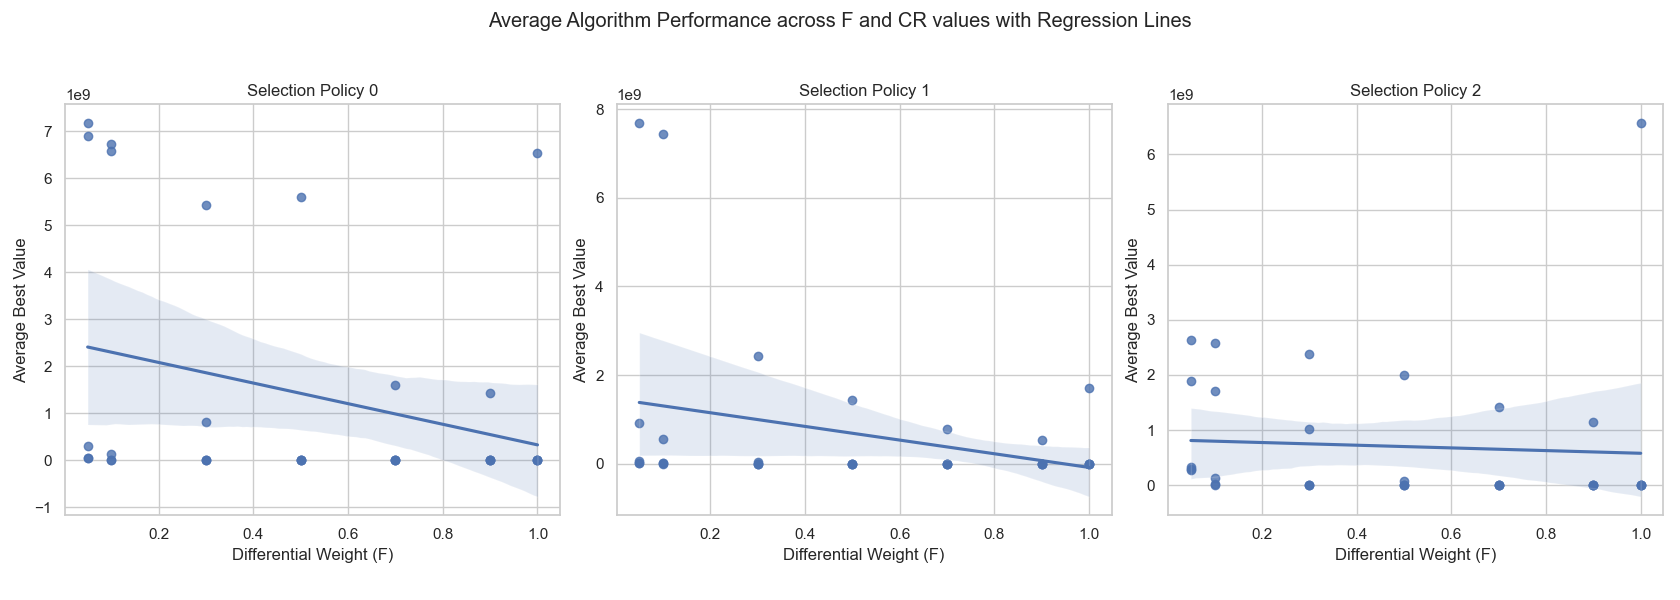
\includegraphics[width=1\textwidth]{Performance_F.png}
    \caption{Performance of algorithms with different values of F. Plot utilizes 40000 examples per dot.}
    \label{fig:f-performance}
\end{figure}

\begin{figure}[h]
    \centering
    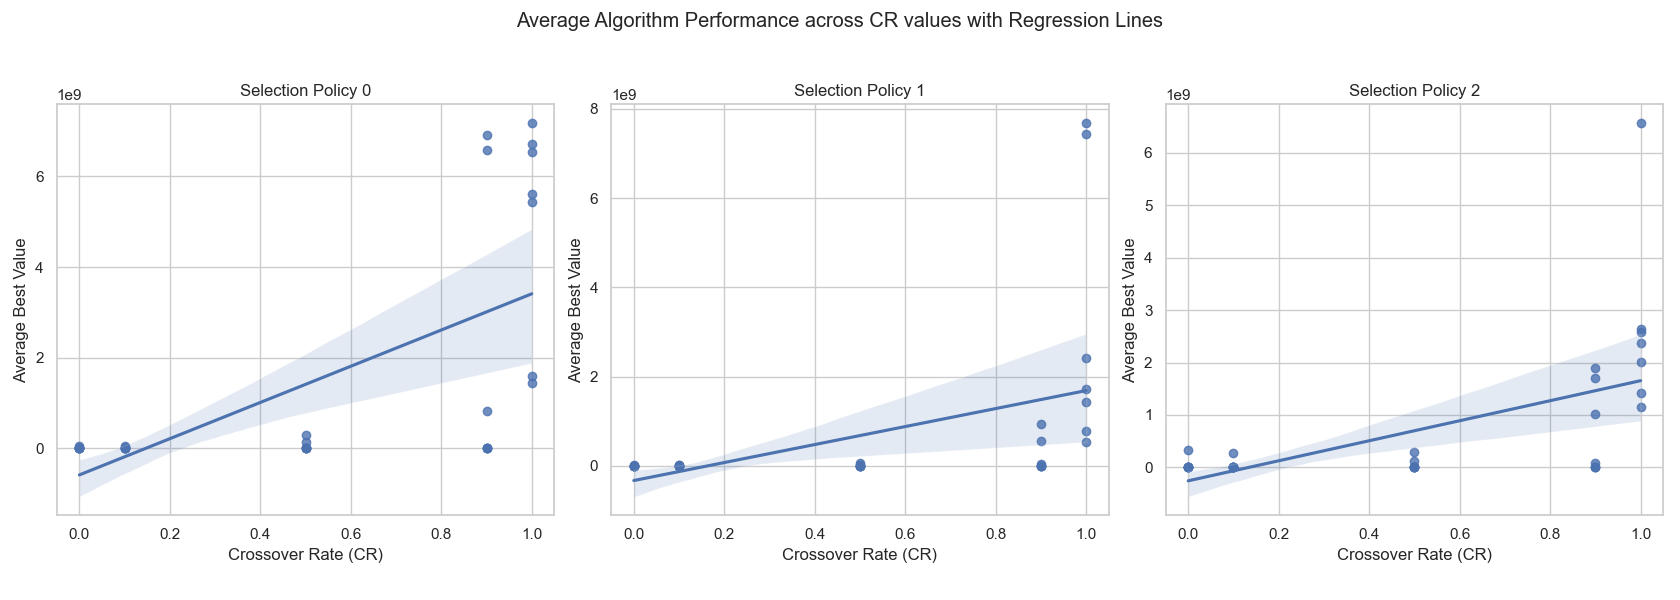
\includegraphics[width=1\textwidth]{Performance_CR.png}
    \caption{Performance of algorithms with different values of CR. Plot utilizes 40000 examples per dot.}
    \label{fig:cr-performance}
\end{figure}

As we can clearly see, performance for higher F is typically increased since the algorithms tend to find optimums better. This however is almost not as evident with the second slection policy which might do with a hybrid evaluation approach.

For the average best result with CR, a lesser CR seems to provide a statistically better value, which actually impressed me quite much. (maybe I did a mistake in calculations. I am not sure)

\textbf{Cohen's d Values:}
\begin{itemize}
    \item Between Policy 0 and 1: 0.065 (small effect size, indicating a minimal practical difference)
    \item Between Policy 0 and 2: -0.156 (small to medium negative effect size, suggesting that Policy 2 might perform slightly worse than Policy 0)
    \item Between Policy 1 and 2: -0.218 (medium negative effect size, indicating a more noticeable underperformance of Policy 2 compared to Policy 1)
\end{itemize}

These statistical measures assist in understanding the statistical significance.

\subsection{Runtime Analysis}
This subsection provides a detailed analysis of the runtime performance of the differential evolution algorithms across various settings of the Differential Weight (F) and Crossover Probability (CR). This analysis is crucial for understanding the computational efficiency of each algorithm configuration under different parameterizations.

\subsubsection{Runtime Variation with Differential Weight and Crossover Probability}
The following figures illustrate how the runtime of algorithms varies with changes in the Differential Weight (F) and Crossover Probability (CR). These plots provide a visual representation of the runtime dynamics that are further quantified in the subsequent table.

\begin{figure}[h]
    \centering
    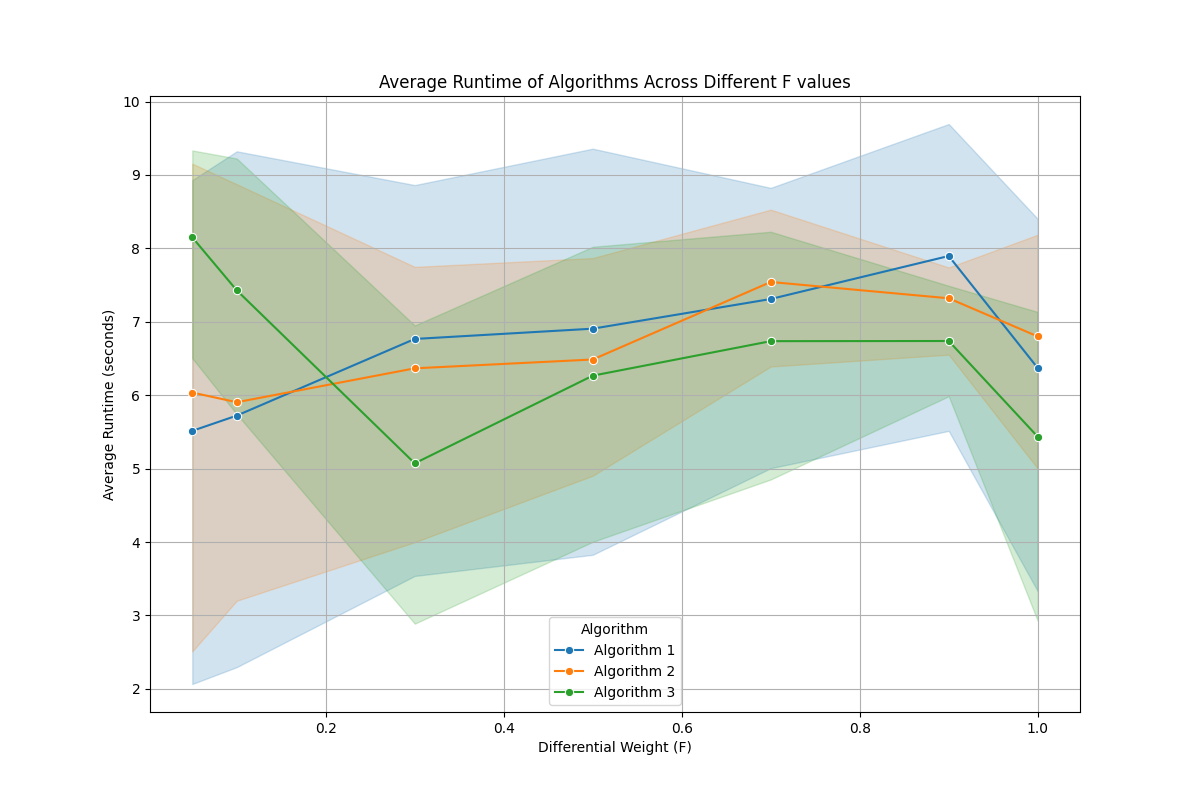
\includegraphics[width=0.7\textwidth]{Runtime_on_various_F.png}
    \caption{Variation of algorithm runtimes with different values of F.}
    \label{fig:runtime-f}
\end{figure}

\begin{figure}[h]
    \centering
    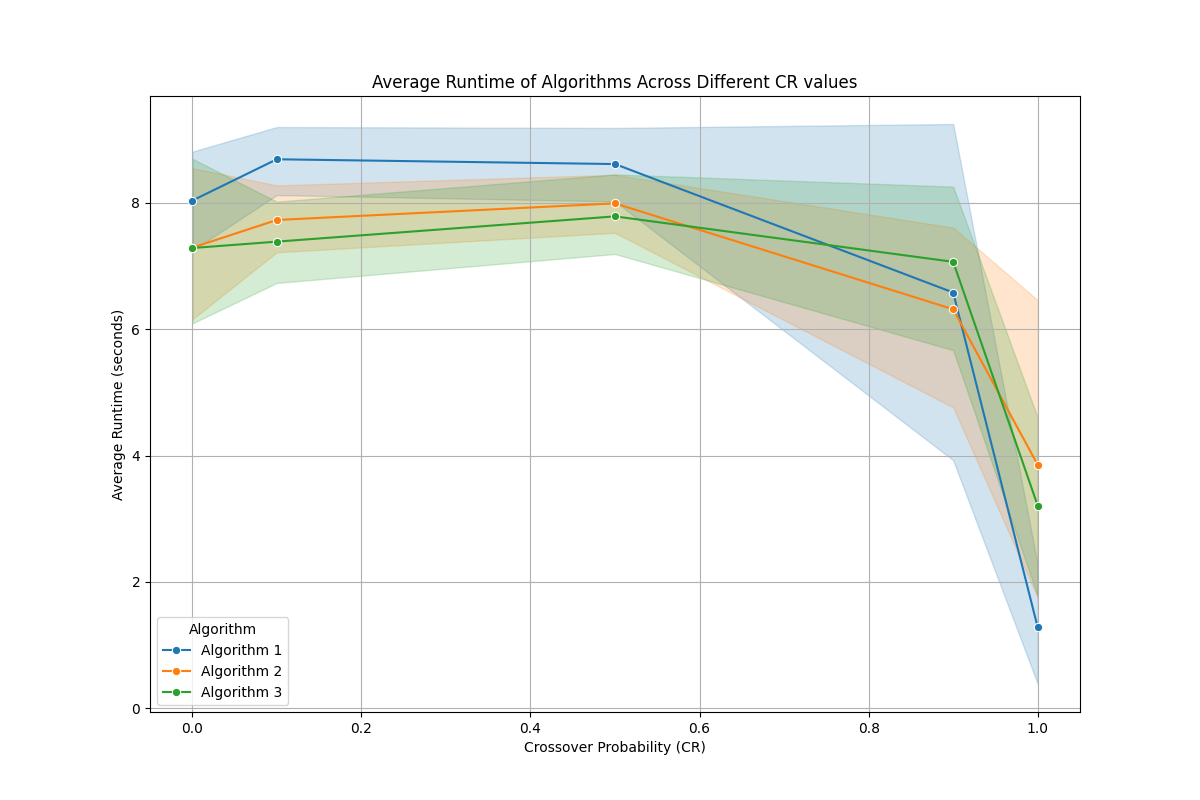
\includegraphics[width=0.7\textwidth]{Runtime_on_various_CR.png}
    \caption{Variation of algorithm runtimes with different values of CR.}
    \label{fig:runtime-cr}
\end{figure}

\subsubsection{Tabulated Runtime Statistics}
The table below provides a detailed breakdown of the average runtimes for each algorithm across various settings of F and CR. Each entry shows the overall runtime, along with individual runtimes for three algorithms, enabling a comparative analysis of performance efficiency.

\begin{table}[h]
    \centering
    \begin{tabular}{ccccccc}
        \hline
        F & CR & Overall (s) & Algorithm 1 (s) & Algorithm 2 (s) & Algorithm 3 (s) \\
        \hline
        0.05 & 0.0 & 333.57 & 9.0 & 9.83 & 9.56 \\
        0.05 & 0.1 & 276.14 & 8.5 & 8.47 & 8.93 \\
        0.05&0.5&263.9&9.15&8.82&7.82 \\
        0.05 & 0.9 & 155.08 & 0.79&2.55&9.31 \\
        0.05&1.0&102.23&0.13&0.51&5.13 \\
        0.1&0.0&368.17&9.73&9.75&10.34 \\
        0.1&0.1&282.12&9.66&6.7&6.05 \\
         ...&...&...&...&...&... \\
        1.0 & 0.0 & 253.21&7.88&6.91&6.75 \\
        1.0 & 0.1 & 289.0&9.41&9.02&7.74 \\
        1.0 & 0.5 & 274.96&7.43&6.96&6.69 \\
        1.0 & 0.9 & 193.59&6.68&7.4&5.54 \\
        1.0 & 1.0 & 38.45 & 0.45 & 3.71 & 0.45 \\
        \hline
    \end{tabular}
    \caption{Average runtime statistics for different algorithms under varying settings of F and CR. More data included in average\_runtimes.csv [2]}
    \label{tab:runtime-stats}
\end{table}

This comprehensive analysis shows that the runtime is influenced by the selection of F and CR parameters, suggesting that optimization of these parameters is essential for improving the efficiency of the algorithms.

\section{Conclusions}
\textbf{Parameter Tuning and Algorithm Performance}: The F and CR parameters significantly influence the performance of DE algorithms. Fine-tuning these parameters can lead to optimal performance, as evidenced by the varying results across different configurations.

\textbf{Statistical Significance}: The use of robust statistical methods, such as the Shapiro-Wilk test, Kruskal-Wallis test, and Dunn's post-hoc test, confirmed the statistical significance of differences in performance between selection policies. These differences underline the importance of careful parameter selection in optimizing DE algorithms.

\textbf{Sample Size and Power Analysis}: Simulations to estimate the required sample size for achieving desired statistical power underscored the importance of sufficiently large datasets. This ensures reliable detection of practical differences between configurations.

\textbf{Outliers and Data Distribution}: Outliers were consistently observed and retained for analysis due to their regular appearance across different parameter settings, suggesting they are inherent to the algorithm's stochastic nature rather than anomalies.

\textbf{Runtime Analysis}: Detailed runtime analysis revealed how the computational efficiency of DE algorithms varies with different F and CR settings. This analysis aids in understanding the trade-offs between runtime and algorithmic performance.

\textbf{Optimal Configurations}: The study identified optimal F and CR settings for each selection policy, providing actionable insights for practical applications of DE algorithms.


\section*{References}
\begin{enumerate}
    \item \textbf{Mamanchuk N., University of Tsukuba}, Github, \today. Available online: \url{https://github.com/RIFLE}
    \item \textbf{Mamanchuk N., University of Tsukuba}, Archive with Results for EDCS, Report 2, 2024. Available online: \url{https://drive.google.com/drive/folders/1IDyFj6jiNZ1P3mERxWX4vkladGiPFlor?usp=drive_link} [Uploaded: 2024-07-16]
    % \item \textbf{Company}, Name of Work, year. Available online: \url{https://...} [Accessed: yyyy-mm-dd]
\end{enumerate}

\newpage

\section*{Appendix A. Listing sample\_size.py} % Any code goes here
\begin{lstlisting}[language=python, title=Showcase of implementation. sample\_size is 1940]
import numpy as np
import scipy.stats as stats

def simulate_kruskal(n, num_groups, effect_size, iterations):
    power_count = 0
    for _ in range(iterations):
        # Create data for each group with some effect
        groups = [np.random.normal(loc=i*effect_size, scale=1, size=n) for i in range(num_groups)]
        _, p_value = stats.kruskal(*groups)
        if p_value < 0.05:
            power_count += 1
    return power_count / iterations

# Set parameters
num_groups = 3  # As per three selection policies
desired_power = 0.8
alpha = 0.05
effect_size = 0.05  # Hypothetical effect size, adjust based on expected differences
iterations = 1000  # More iterations, more accurate power estimation

# Estimate required sample size
sample_size = 10  # Start with a low number
while True:
    power = simulate_kruskal(sample_size, num_groups, effect_size, iterations)
    print(f"Sample size: {sample_size}, Estimated Power: {power}")
    if power >= desired_power:
        break
    sample_size += 5

print(f"Required sample size to achieve {desired_power*100}% power is approximately {sample_size}")
\end{lstlisting}

\newpage
\section*{Appendix B. Listing record\_performance\_and\_runtime.py}
\begin{lstlisting}[language=python, title=Showcase of implementation. Files are recorded using all\_stats.py.]
import os
import pandas as pd

def analyze_performance(directory, file_name):
    file_path = os.path.join('results', directory, 'best', file_name)
    data = pd.read_csv(file_path)
    runtime_info = data.iloc[-1, 0]  # Extract runtime information
    data = data.iloc[:-1]  # Remove the last info row
    min_best = data.groupby('Selection Policy')['best'].min().reset_index()
    return min_best, runtime_info

def extract_runtime_info(runtime_str):
    parts = runtime_str.split(',')
    runtime = {
        'overall': float(parts[3].split(':')[1].strip().split(' ')[0]),
        'alg1': float(parts[4].split('=')[1].strip('s')),
        'alg2': float(parts[5].split('=')[1].strip('s')),
        'alg3': float(parts[6].split('=')[1].strip('s'))
    }
    return runtime

# List of all directories and files
configurations = [
    {"dir": "20240716145045-8-194-0.05-1", "file": "resultbest_20240716145045.csv"},
    {"dir": "20240716143339-8-194-0.1-1", "file": "resultbest_20240716143339.csv"},
    {"dir": "20240716143827-8-194-0.3-1", "file": "resultbest_20240716143827.csv"},
    {"dir": "20240716144045-8-194-0.5-1", "file": "resultbest_20240716144045.csv"},
    {"dir": "20240716144207-8-194-0.7-1", "file": "resultbest_20240716144207.csv"},
    {"dir": "20240716144534-8-194-0.9-1", "file": "resultbest_20240716144534.csv"},
    {"dir": "20240716144847-8-194-1-1", "file": "resultbest_20240716144847.csv"},
    {"dir": "20240716145310-8-194-0.05-0.9", "file": "resultbest_20240716145310.csv"},
    {"dir": "20240716145612-8-194-0.1-0.9", "file": "resultbest_20240716145612.csv"},
    {"dir": "20240716145906-8-194-0.3-0.9", "file": "resultbest_20240716145906.csv"},
    {"dir": "20240716150244-8-194-0.5-0.9", "file": "resultbest_20240716150244.csv"},
    {"dir": "20240716150658-8-194-0.7-0.9", "file": "resultbest_20240716150658.csv"},
    {"dir": "20240716151149-8-194-0.9-0.9", "file": "resultbest_20240716151149.csv"},
    {"dir": "20240716151700-8-194-1-0.9", "file": "resultbest_20240716151700.csv"},
    {"dir": "20240716155602-8-194-0.05-0.5", "file": "resultbest_20240716155602.csv"},
    {"dir": "20240716155052-8-194-0.1-0.5", "file": "resultbest_20240716155052.csv"},
    {"dir": "20240716154521-8-194-0.3-0.5", "file": "resultbest_20240716154521.csv"},
    {"dir": "20240716154006-8-194-0.5-0.5", "file": "resultbest_20240716154006.csv"},
    {"dir": "20240716153246-8-194-0.7-0.5", "file": "resultbest_20240716153246.csv"},
    {"dir": "20240716152736-8-194-0.9-0.5", "file": "resultbest_20240716152736.csv"},
    {"dir": "20240716152245-8-194-1-0.5", "file": "resultbest_20240716152245.csv"},
    {"dir": "20240716160103-8-194-1-0.1", "file": "resultbest_20240716160103.csv"},
    {"dir": "20240716160604-8-194-0.9-0.1", "file": "resultbest_20240716160604.csv"},
    {"dir": "20240716161151-8-194-0.7-0.1", "file": "resultbest_20240716161151.csv"},
    {"dir": "20240716161808-8-194-0.5-0.1", "file": "resultbest_20240716161808.csv"},
    {"dir": "20240716162356-8-194-0.3-0.1", "file": "resultbest_20240716162356.csv"},
    {"dir": "20240716162912-8-194-0.1-0.1", "file": "resultbest_20240716162912.csv"},
    {"dir": "20240716163616-8-194-0.05-0.1", "file": "resultbest_20240716163616.csv"},
    {"dir": "20240716164204-8-194-1-0", "file": "resultbest_20240716164204.csv"},
    {"dir": "20240716164826-8-194-0.9-0", "file": "resultbest_20240716164826.csv"},
    {"dir": "20240716165344-8-194-0.7-0", "file": "resultbest_20240716165344.csv"},
    {"dir": "20240716165822-8-194-0.5-0", "file": "resultbest_20240716165822.csv"},
    {"dir": "20240716170310-8-194-0.3-0", "file": "resultbest_20240716170310.csv"},
    {"dir": "20240716170844-8-194-0.1-0", "file": "resultbest_20240716170844.csv"},
    {"dir": "20240716171551-8-194-0.05-0", "file": "resultbest_20240716171551.csv"},
]

best_performances = {}
runtime_data = []

for config in configurations:
    best_data, runtime_info = analyze_performance(config['dir'], config['file'])
    runtime = extract_runtime_info(runtime_info)
    runtime['F'] = config['dir'].split('-')[3]  # Extract F value
    runtime['CR'] = config['dir'].split('-')[4]  # Extract CR value
    runtime_data.append(runtime)
    
    for index, row in best_data.iterrows():
        policy = int(row['Selection Policy'])
        best_score = row['best']
        if policy not in best_performances or best_score < best_performances[policy]['best_score']:
            best_performances[policy] = {
                'best_score': best_score,
                'F': config['dir'].split('-')[3],
                'CR': config['dir'].split('-')[4]
            }

# Create dataframes from the performance and runtime data
performance_df = pd.DataFrame.from_dict(best_performances, orient='index')
runtime_df = pd.DataFrame(runtime_data)

# Save the performance data to a CSV file
performance_df.to_csv('performance_stats.csv', index_label='Selection Policy')
print("Performance statistics saved to 'performance_stats.csv'")

# Save the runtime data to another CSV file
runtime_df.to_csv('runtime_stats.csv', index=False)
print("Runtime statistics saved to 'runtime_stats.csv'")    
\end{lstlisting}

\newpage

\section*{Appendix C. Interbenchmark Host Hoc Dunn Performance}
\begin{figure}[h]
    \centering
    \includegraphics[scale=0.8]{results/20240716062920-8-194-0.7-0.5/all/posthoc-heatmaps/20240716062920-8-194-0.7-0.5_P7.0_hosthoc_heatmap.png}
    \caption{Results showcase for PH analysis for 20240716062920-8-194-0.7-0.5\_P7.0\_hosthoc\_heatmap.png} 
\end{figure}

% #################### ENDING HERE ####################

\end{document}
